% Chapter 1

\chapter{Introduction} % Main chapter title
%\addchaptertocentry{Introduction} 
\label{Introduction} % For referencing the chapter elsewhere, use \ref{Chapter1} 

%----------------------------------------------------------------------------------------

% Define some commands to keep the formatting separated from the content 
\newcommand{\keyword}[1]{\textbf{#1}}
\newcommand{\tabhead}[1]{\textbf{#1}}
\newcommand{\code}[1]{\texttt{#1}}
\newcommand{\file}[1]{\texttt{\bfseries#1}}
\newcommand{\option}[1]{\texttt{\itshape#1}}

%----------------------------------------------------------------------------------------

\section{Vision naturelle}
>> Rôle de la vision\\
Tous  les êtres vivants utilisent la vision à un degré ou à un autre, et pour de nombreuses espèces -y compris la notre- elle est même la modalité perceptive principale. Chez nous, cette dominance de la vision transcende la notion de modalité perceptive et s'ancre dans notre culture, que ce soit au travers des arts ou du language (qui n'a jamais dit un jour ''Ah, je vois!'') ainsi que dans la construction de nos relations sociales, nous permettant de capter ou d'exprimer émotions et intentions.\\

>> Structure générale d'une rétine (cônes/bâtonnets + fovéa/rétine périphérique)\\
Chez les vertébrés la vision débute à la surface de la rétine, où les cellules photovoltaïques (cônes et bâtonnets) réalisent la transduction des signaux lumineux qui les atteignent en signaux électriques, transmissibles à la suite du réseau nerveux.\\
Les cônes et les bâtonnets sont différenciées par un certain nombre de caractéristiques, notamment leur sensibilité aux longueurs d'ondes lumineuses et leur distribution au sein de la rétine. Ces différences permettent à notre rétine de rester fonctionnelle dans de nombreuses situations, y compris lorsque la luminance est très faible (le seuil absolu de la rétine humaine correspondant à 70 photons) et permet donc à la modalité visuelle de nous fournir des informations pertinentes dans un large champs de contextes.\\
Les bâtonnets sont plus nombreux que les cônes et sensibles à des variations de luminance plus fines. Ils sont majoritairement responsables de notre vision scotopique (dans des conditions de faible luminance, tel que la nuit) et sont des acteurs majeurs de la vision périphérique.\\
Le champs visuel peut être divisé en vision centrale et vision périphérique. La vision centrale (environ \SI{2}{\degree}) est soutenue par la région rétinienne appelée fovea, comprenant uniquement des cônes. On y observe l'acuité visuelle la plus importante (la région présente les champs récépteurs les plus petits de la rétine). Cette acuité visuelle diminue avec l'excentricité par rapport à la fovéa (autrement dit, les champs récépteurs visuels grandissent avec cette excentricité ; \cite{Werner2014}).\\

>> Notion de saccades oculaires/Vision d'une cible en périphérie\\
Lors de l'exploration de son environnement visuel, un agent va en conséquence réaliser des saccades oculaires : mouvements brefs (20-60\si{\milli\second}) des globes oculaires (réalisés grâce aux muscles oculomoteurs les encadrant) afin de placer l'image d'une cible (ou sa position prédite dans l'espace) au niveau de la fovéa, permettant ainsi de traiter les informations en provenant avec la plus grande préçision possible.\\

>> Cellules parvo/magno -> rôle de la voie magno\\
L'activité rétinienne est transmise le long des voies nerveuses visuelles jusqu'au cortex visuel, où sera réalisé la majorité du traitement des informatiques qu'elle supporte. \\
Entre la rétine et le cortex existe un certain nombre d'étapes, mais tout au long de ces voies, la distribution rétinienne de l'information  (la rétinotopie) est conservée. 

\begin{figure}[th]
\centering
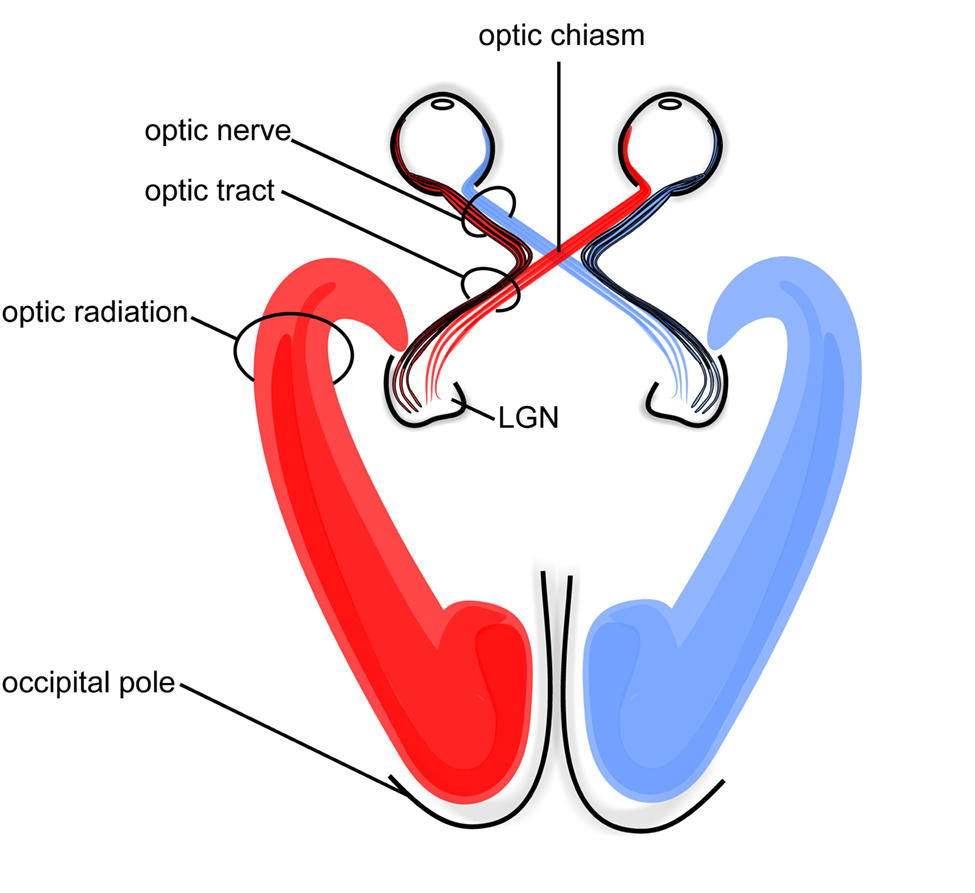
\includegraphics{Figures/visual_system}
\decoRule %puts an aesthetic horizontal line below the image
\caption[Figure]{Schéma des voies visuelles humaines, de la rétine jusqu'au cortex visuel primaire (adapté de Hofer S. et al., 2010 via Wikimedia Commons [CC BY 3.0]})
\label{fig:visual_system}
\end{figure}

Dans leurs travaux de 1962 et 1977, Hubel et Wiesel émettent l'hypohèse des courants visuels, qui définit trois voies visuelles naissant dans le \textbf{corps genouillé latéral} (LGN, où sont présents les corps des types cellulaires donnant leur nom aux voies) et le \textbf{cortex visuel primaire} (V1) :  \textbf{magnocellulaire} (M),  \textbf{parvocellulaire} (P) et  \textbf{koniocellulaire} (K). Chacune supporte le transport d'informations visuelles présentant des caractèristiques distinctes.\\
L'activité des cellules M ne distingue les couleurs et est sensible à des différences fines de luminance, de contraste et de fréquence spatiale. Ces caractèristiques semblent lier la voie M au traitement de la luminance et des mouvements (\cite{Werner2014}).

>> Voie dorsale, rôle dans la localisation de cible et les saccades oculaires\\
La différentiation des voies visuelles est conservée au delà de V1, et l'on décrit alors deux voies visuelles :  \textbf{dorsale} (codant majoritairement pour des informations provenant de la voie M) et  \textbf{ventrale} (codant majoritairement pour des informations provenant de la voie P).\\
La voie centrale communique ainsi principalement avec les aires cérébrales du lobe temporal, l'activité de son réseau étant primordiale pour la reconnaissance et l'identification des objets visuels. La voie dorsale quant à elle communique principalement avec les aires du lobe pariétal, l'activité de ce réseau étant primordiale pour le traitement des relations spatiales entre les objets visuels ainsi que pour le guidage attentionnel et physique vers eux (\cite{Werner2014}).\\
Parmi ce réseau dorsal, on trouve l'\textbf{aire intrapariétale latérale} (LIP) et l'aire 7a, qui recoivent en partie des informations directement depuis V1 et V2 (contournant donc le traitement d'aires en amont, dont l'aire MT) codant pour des stimuli dans le champs visuel périphérique.\\
Plus spécifiquement, des travaux ont relié l'activité des neurones de l'aire LIP à la plannification des saccades oculaires et à la représentation spatiale des objets visuels.

%----------------------------------------------------------------------------------------

\section{Vision artificielle}
>> Motivations\\
Valider l'une des théories neurofonctionnelles de la détection de cible visuelle.\\
Construire un modèle de vision artificielle, pouvant à maturité être intégré dans des systèmes embarqués. L'approche biomimétique permet de répondre à un certain nombre de contraintes de ces systèmes, notamment en terme de poids numérique, de puissance de calcul disponible et d'adaptabilité.\\

\begin{equation}
E = mc^{2}
\label{eqn:Einstein}
\end{equation}

If you don't want a particular equation numbered, use the unnumbered form:
\begin{verbatim}
\[ a^{2}=4 \]
\end{verbatim}
